\section{Implementation}\label{sec:impl}

Our \tube system has two components; the tube itself and the screen. As shown in Figure~\ref{fig:impl1}, the tube is attached to an acrylic enclosure that houses a small Force-Sensing Resistor (FSR) and an Inertial Measurement Unit (IMU). The IMU captures the three-dimensional motion of the tube and translates it into 2-dimensional position on the screen. Additionally, it also records the angle in which the tube is rotated and how fast it is rotating. With the FSR integrated in the tube, the magnitude of the user’s breathing into the tube is also captured. 

\begin{figure}
  \centering
  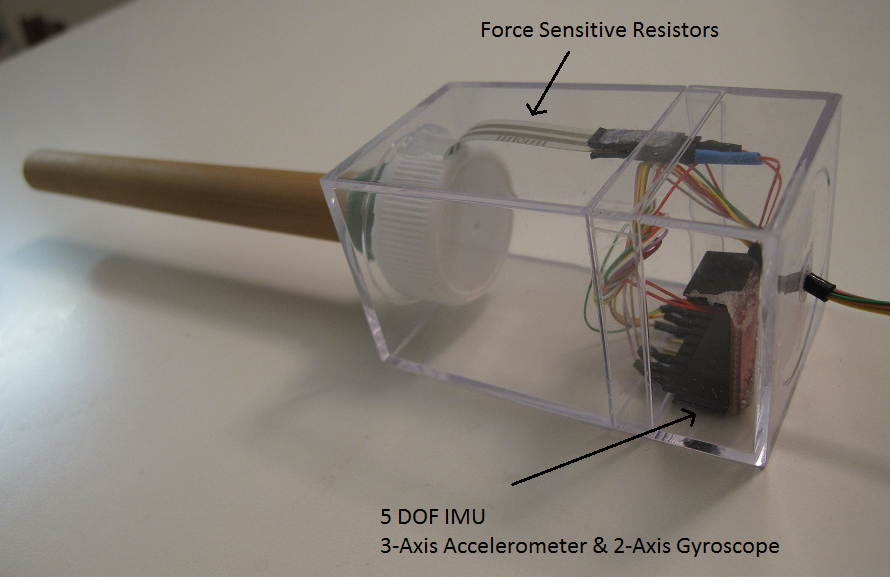
\includegraphics[width=\linewidth]{./figs/impl1.png}
  \caption{Our \tube with all the sensors.}
  \label{fig:impl1}
\end{figure}

Figure~\ref{fig:design-sketch} shows an overview of how our \tube system works as a whole. As we move or rotate \tube, our movements are recorded by an Arduino microcontroller. Arduino will then send all of the data it received to be used by the applications in the computer which is then displayed in an output system such as computer screen.

\begin{figure}
  \centering
  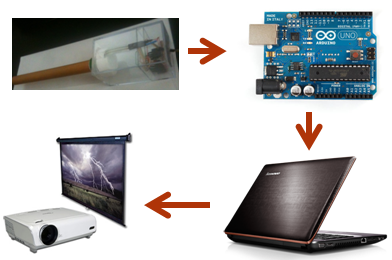
\includegraphics[width=0.8\linewidth]{./figs/sketch.png}
  \caption{Overview of how our system works.}
  \label{fig:design-sketch}
\end{figure}

We have developed two applications that demonstrate the uniqueness and interactiveness of our \tube. The applications that we developed are written in processing since it provides a smooth interface with Arduino while boasting numerous easy-to-use graphical functions. Additionally, making existing processing applications to work with our \tube requires very minimal changes to their code base since we have made the interface to the hardware very simple and generic.

\subsection{\textbf{Painting Application}}

Our first application is a painting application program. In this application, the user will be able to paint by blowing into the tube and the harder the user blows, the thicker the paint will be. Changing the color of the paint is achieved by rotating the tube. We implemented the strokes to be brush-like, as if the user is painting with a real brush.

\begin{figure}
  \centering
  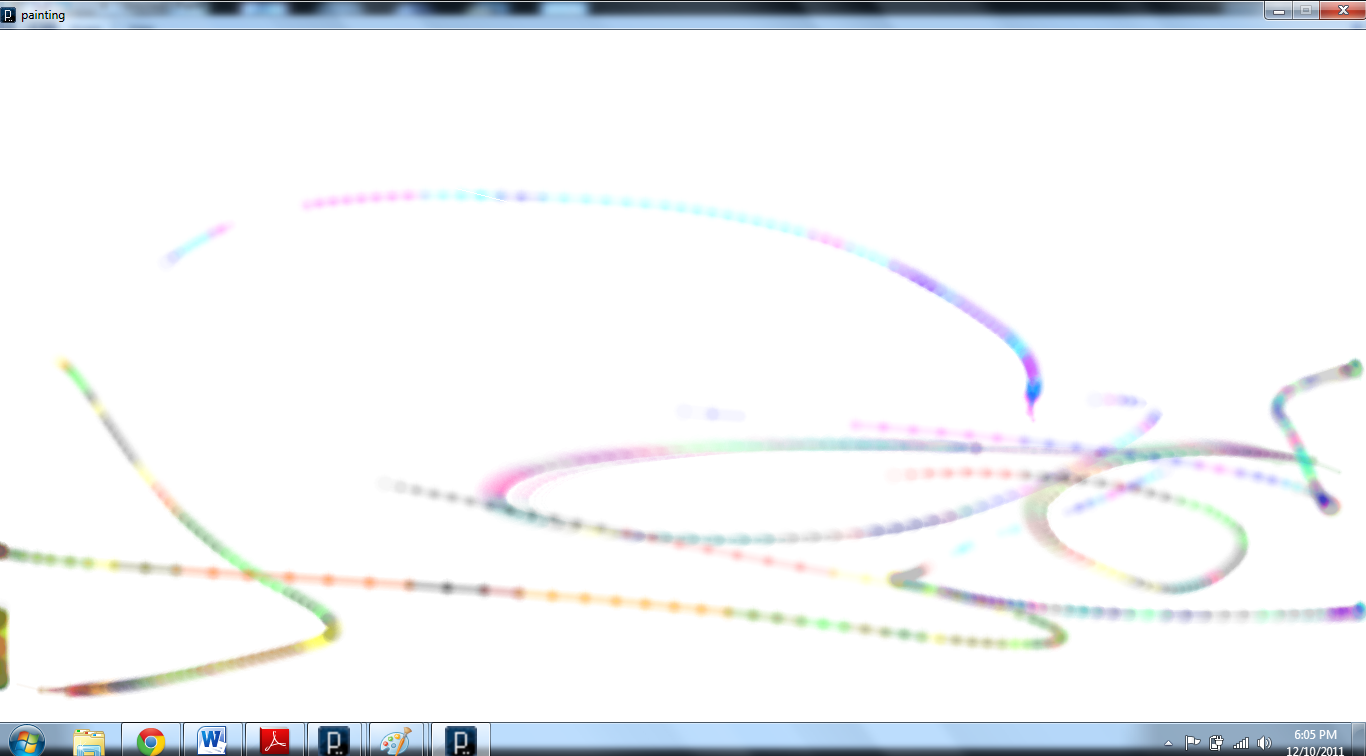
\includegraphics[width=\linewidth]{./figs/tube3.png}
  \caption{A screenshot of our painting application, drawn by our tester.}
  \label{fig:painting}
\end{figure}

\subsection{\textbf{Balloon Popping Game}}

The next application is a game in which the user is required to pass through a set of levels by popping the balloons that randomly appear on the screen, as shown in Figure~\ref{fig:shooting-game}. This is done by moving the pointer to where the balloons are and blowing into the tube. The game consists of two levels: in the first level, the pointer and the balloons' color are all black so that user only needs to point and shoot. This level is intended to familiarize the user with the basic concept of controlling the movement of our \tube to achieve the desired objective. In the second level, the colors of the generated balloons are randomly chosen between red, blue and green. For the user to be able to pop the balloons, the user will have to match the color of the pointer and each balloon by rotating the tube before blowing into the tube.

\begin{figure}
  \centering
  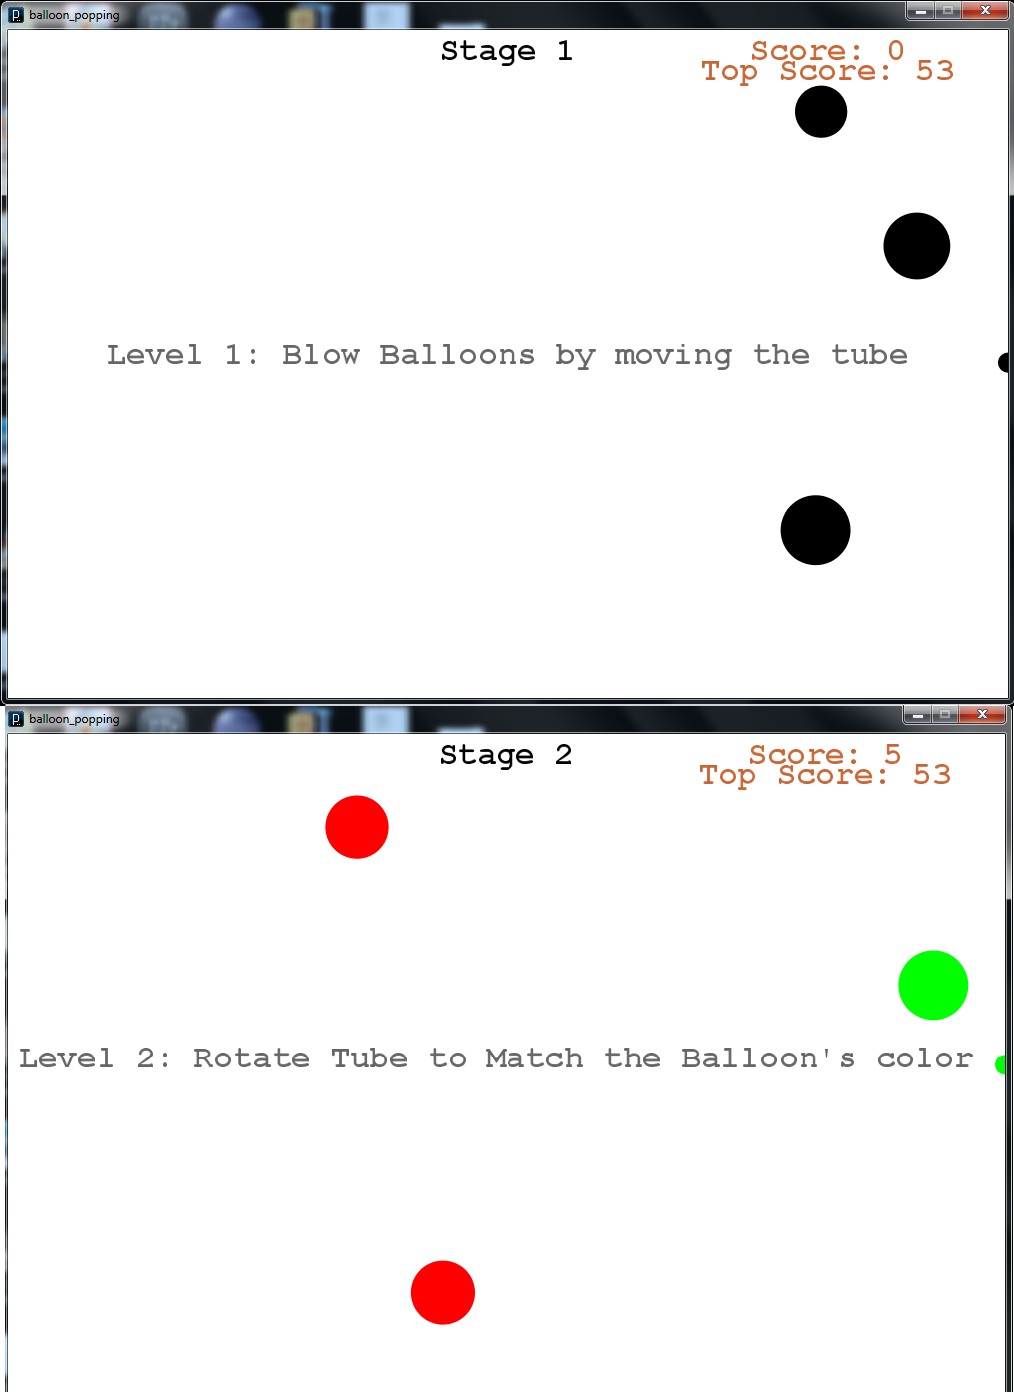
\includegraphics[width=0.70\linewidth]{./figs/tubemaster.png}
  \caption{A screenshot of the beginning of each level of our balloon popping game.}
  \label{fig:shooting-game}
\end{figure}

